\documentclass{report}
\usepackage{setspace} % Setting line spacing
\usepackage{ulem} % Underline
\usepackage{caption} % Captioning figures
\usepackage{subcaption} % Subfigures
\usepackage{geometry} % Page layout
\usepackage{multicol} % Columned pages
\usepackage{array,etoolbox}
\usepackage{fancyhdr}
\usepackage{enumitem}
\usepackage[toc,page]{appendix}
\setlist{noitemsep}

%READ THIS:
%mark comments with OpenComment or ClosedComment as you write, so we can ctrl+f as needed.

% Page layout (margins, size, line spacing)
\geometry{letterpaper, left=1in, right=1in, bottom=1in, top=1in}
\setstretch{1}

% Headers
\pagestyle{fancy}
\lhead{PeaPod - Design Report}
\rhead{UTAG}

\begin{document}

\begin{titlepage}
    \begin{center}
        \vspace*{1.2cm}

        \textbf{\large{PeaPod - Design Report}}

        \vspace{0.5cm}

        Primary Written Deliverable for the Deep Space Food Challenge Phase 1

        \vfill \small{

            \textbf{Jayden Lefebvre - Lead Engineer, UTAG Founder}\\
            BASc Computer Engineering (Anticipated 2024), University of Toronto\\
            Toronto, ON, Canada\\
            \vspace{.5cm}
            \textbf{Nathan Chareunsouk - Design Lead}\\Toronto, ON, Canada\\
            \vspace{.5cm}
            \textbf{Navin Vanderwert - Design Engineer}\\
            BASc Engineering Science (Anticipated 2024), University of Toronto\\
            Toronto, ON, Canada\\
            \vspace{.5cm}
            \textbf{Jonas Marshall - Electronics Engineer}\\
            BASc Computer Engineering (Anticipated 2024), Queen's University\\
            Kingston, ON, Canada

        }

        \vspace{1cm}

        Primary Contact Email: jayden.lefebvre@mail.utoronto.ca

        \vspace{.75cm}

        Revision 0.6\\
        University of Toronto Agritech\\
        July 28th, 2021

    \end{center}
\end{titlepage}

\thispagestyle{plain}

\tableofcontents
\newpage

\section{Design Abstract}
% Please provide a brief summary description of your proposed food production technology within a 1,500 character limit. The abstract may answer some of the following questions: What is your proposed solution? What is novel, sustainable, and innovative about your proposed solution? What types of food does your solution create? How are you minimizing inputs and maximizing food outputs?

PeaPod is a precision-automated plant growth environment, designed as both a low-maintenance modular food production system and a distributed research tool. PeaPod is able to generate any desired environment to grow any crop, while collecting data on plant growth to optimize food products over time.

The growth environment is extendable and modular, and is easily adapted to suit plant selection and mission requirements. The housing consists of a "unit cell" cube skeleton, repeated upwards and sideways to expand the environment. The housing is then insulated with internally-reflective panels for greater efficiency.

PeaPod uses a set of control systems to generate the desired environment. Systems include air thermoregulation, humidification, dehumidification LED lighting and an aeroponics system. These systems are fully automated by an onboard computer and housed in a self-contained control module mounted to the top of the housing. This allows control power to be multiplied in larger extended PeaPods by adding more control modules in a controller-follower topology.

Both plant growth platforms as well as lighting systems are built on modular "tray" subframes mounted to the inside of the housing, enabling the user to add, remove, or reposition plants and lights at will to accommodate any plant size.

Throughout each growth cycle iteration, PeaPod collects data on all environment parameters and plant metrics. This data is then used to train a machine learning model to represent the plant's phenology across time in the given environment. This model produces a function, which can then be optimized for yield Mass, nutrient concentration, flavour, energy efficiency, water use, or any other metric. Therefore plants grown in PeaPod will be more nutritious, taste better, and yield more as more iterations are performed.

Combining all these features into an accessible open-source design, PeaPod provides unrivalled versatility and reliability to food production systems both terrestrially and on long-duration space missions.

\section{Design Report}

\subsection{Description}
\label{sec:description}

\textbf{Part A}
\label{sec:description-a}

% ===== PROMPT =====

% Please provide a more fulsome description of your food production technology. Your description needs to include information about what the technology is, what it does, how it functions, and how the crew will interact with it. Be sure to also provide any descriptions of major hardware components and processes in relation to your technology.

% ===== WRITE =====
% 3000chars

PeaPod is a precision-automated plant growth environment, designed as both a low-maintenance food production system and a distributed research tool. PeaPod is able to generate any desired environment, while collecting data on plant growth and improving yields over time.

PeaPod accomplishes this via a number of control systems, some of which are feedback-based (sensor + actuator control loop):

\begin{itemize}
    \item\textit{Lighting}: A wide spectral range (near-ultraviolet$\to$near-infrared) of powerful LEDs, with dimmable drivers for precision spectrum and intensity control. LEDs chosen for high energy efficiency, precise emission spectrum, low heat production, and low risk of plant tissue damage.
    \item \textit{Aeroponics}: Reverse osmosis water is pressurized by a pump and tank. Pressurized water flows through a thermoelectric water block to be heated or cooled, with temperature and pressure sensors providing Proportionate-Integral-Derivative (PID) feedback and safety cutoffs respectively. This is followed by an injection manifold, where parallel Venturis siphon different nutrient and pH adjustment solutions from containers for inline mixing. Servo-actuated flow-control valves control injection rates. The mixed solution now flows through a solenoid to nozzles mounted beneath the plant support trays, enclosed in a water-tight chamber. Runoff water is pumped from the chamber basin and recycled to the injection manifold. Both runoff and supply lines are quick-disconnect for easy tray removal. This method is chosen for increased water efficiency (98\% less than farming), no pH/nutrient "feedback" loop (common in hydroponics), greater supported crop variety (vs hydroponics).
    \item \textit{Air Thermoregulation}: Leaf zone air temperature is regulated by a thermoelectric heat pump. Thermoelectric/Peltier tiles heat or cool an internal heat sink (via thermal compound). Circulation fans blow air over the heat sinks to distribute heat to homogenously heat or cool the environment. A matching heat sink and fan set on the opposite face of the Peltier tiles conduct heat to/from surroundings, completing the heat pump. A PID control system is informed by temperature sensors distributed throughout the growth environment, and - with the use of a MOSFET H-bridge and dimmable current source - controls the direction and magnitude of the heat transfer. This method is chosen for its low complexity (no liquids, pressurization, etc.) and ease of automation (bidirectional heat pump, precisely dimmable, PID tuning for high accuracy).
    \item \textit{Humidity Regulation}: Leaf zone humidity is regulated by two complementary systems. A dead-zone bang-bang control system is informed by humidity sensors distributed throughout the growth environment.
    \begin{itemize}
        \item \textit{Humidification}: Humidity is \textbf{increased} by an ultrasonic mesh nebulizer. Reverse osmosis water is supplied to a small container, to which a piezoelectric mesh disc is mounted. A control signal activates a driver circuit which causes the disc to oscillate, producing water vapour. This method is chosen for its ease of automation and consistency of vapour production.
        \item \textit{Dehumidification}: Humidity is \textbf{decreased} by a rechargeable indicating desiccant cartridge. The cartridge, containing dry silica gel beads, is inserted into a housing. Servo-actuated "shutters" prevent unintended air movement through the cartridge. Fans draw humid air through a HEPA filter into the cartridge, causing dry air to be expelled back into the growth environment. The cartridge changes color to indicate saturation, which is observed by the automation controller. The crew is then notified to swap the saturated cartridge for a dry one, and to "recharge" the cartridge via evaporation in a standard oven.
    \end{itemize}
    \item \textit{Aeroponic Water Temperature}: Root zone air temperature is regulated in the same way as the leaf zone system. Exceptions include the use of an aluminum water block (as opposed to an internal heat sink and fan) and a single temperature sensor mounted \textbf{after} to account for flow direction.
    \item \textit{Gas Composition}: Oxygen and carbon dioxide concentration imbalances due to photosynthesis are managed by gas exchange with the surroundings. Two ports are covered by servo-actuated "shutters", preventing unintended exchange. Fans draw outside air in via an input port, bringing CO${}_2$ up and O${}_2$ down. Fans also draw inside air out to an onboard filtration and dehumidification system, filtering out aerosols (pollen, seeds, allergens, etc.) and bringing humidity down to acceptable levels. Gas concentration sensors collect data on the concentrations of relevant gasses (CO${}_2$, O${}_2$, etc.), informing a bang-bang control system for the input and output port shutters and fans. This approach allows natural photosynthesis to counteract human carbon dioxide production while remaining safe and minimizing cross-contamination.
\end{itemize}

Food products are optimized over time via plant metric analysis and "surrogate model" machine learning. Cameras (birds-eye and horizontal) capture live video for observation as well as time lapse photography for computer vision analysis. Metrics of both plant health and yield quality (plant "output"), along with data collected on the environment (plant "input"), are used to train a machine learning model to act as a digital representation of the plant. As more iterations of the plant are grown, the dataset becomes generalized across different environmental inputs/programs, and new programs can be selected to intelligently target certain optimization factors (i.e. yield mass, flavour, nutrient concentration, energy/water efficiency).

% Together, these 4 components create the "Black Box" seen in Figure \ref{fig:blackbox}.

% \begin{figure}[h]
%     \centering
%     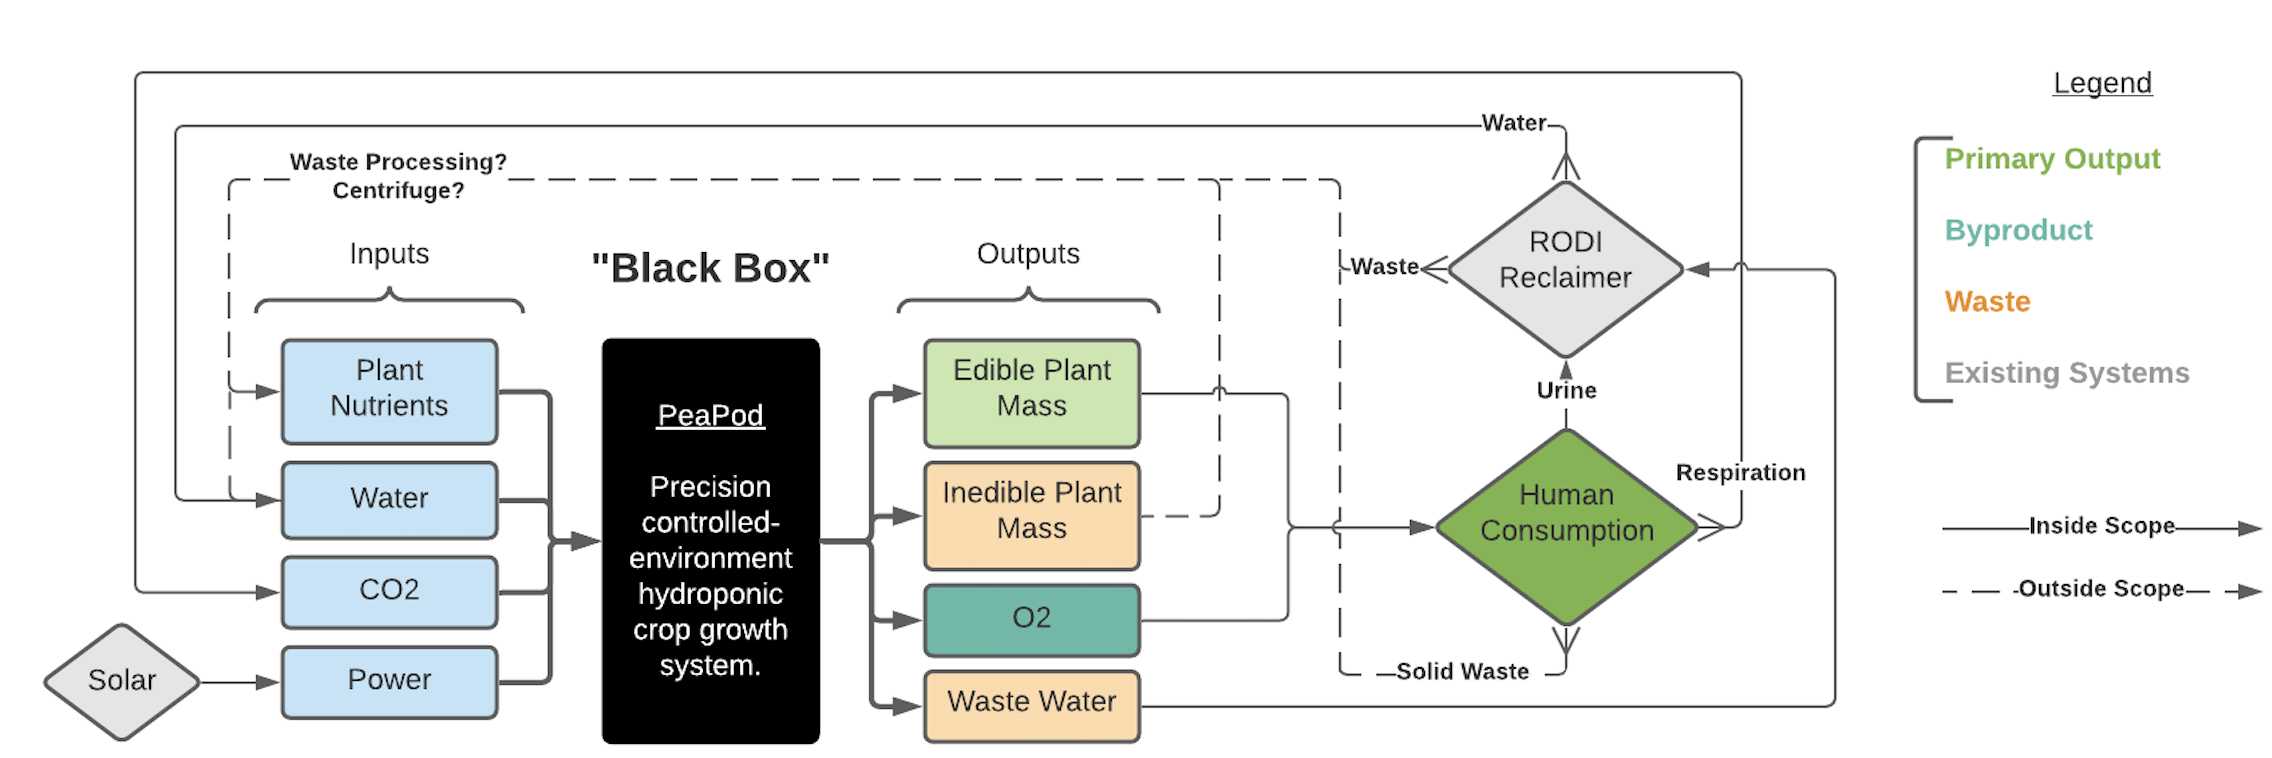
\includegraphics[width=15cm]{../solutionoverview/images/blackbox.png}
%     \hfill
%     \caption{"Black box" function diagram for our solution.}
%     \label{fig:blackbox}
% \end{figure}

\textbf{Part B:}
\label{sec:description-b}

% ===== PROMPT =====

% Please describe the basic operations concept of the food production technology. In your response, describe assumptions required of operation. You can also include, for example, details about whether a sterile/aseptic environment is needed, if special steps are required between production cycles, or if fluids or materials must be removed or added to prime/inoculate a system.

% ===== WRITE =====
% 1500chars

PeaPod's primary function of plant growth is accomplished by achieving total environmental control. 

Once PeaPod has been assembled, the first step is sterilization. Since growth environments may experience high humidities, manual sterilization of the internal environment is necessary to prevent microbial growth. Any plant- and food-safe means may be employed (i.e. UV).

After sterilization, input hookup/filling, and initialization, PeaPod's operation begins at planting. Seeds (or offshoots/clones) are removed from sealed storage bags and placed in neoprene foam "pucks" known as clone collars, which are moistened for germination and placed in the grow cups. The front panel is then closed, sealing the internal environment.

The state of the growth environment is encoded via a standardized set of "environment parameters". The specific values of each parameter for each iteration are stored in a "program". The program is set prior to the start of plant growth, and consists of a set of \textbf{actions} (e.g. set red LEDs to 63\% power) and \textbf{control targets} (e.g. hold air temperature at 22°C) as time-series instructions from the start of planting to the point of harvest (or plant death, in the case of multiple-harvest plants).

Environment parameters:
\begin{itemize}
    \item Leaf zone temperature;
    \item Root zone temperature;
    \item Leaf zone humidity;
    \item Air gas composition;
    \item Light intensity and spectrum;
    \item Aeroponic delivery schedule (timings and durations);
    \item Aeroponic nutrient concentrations;
    \item Aeroponic pH;
\end{itemize}

The environment can be adjusted live by crew or remotely at any point; this is recorded as new instruction entries in the program. In addition, cameras in the environment allow crew to monitor plant growth live.

When activated, PeaPod's control systems begin to enact the program. PeaPod will periodically notify crew of required action, including refilling inputs, cleaning components, and harvesting, as well as notifying upon "End-of-Program", when all inedible plant matter is disposed of. The process can then be repeated (starting at sterilization).

PeaPod leverages existing life support systems for providing inputs and handling outputs.

\textit{Infrastructural Inputs}: Reverse osmosis water (onboard RODI system), nutrient solutions (stored), pH solutions (stored), power (onboard power), network connection (onboard network), plant seeds/clones (stored), input air

\textit{Process Inputs}: Plant species identifiers, environment program, nutrient and pH-adjustment solution identifiers (compounds and molarities, i.e. solution A is 0.6M NaNO${}_3$)

\textit{Products}: Edible plant matter, recorded environment data, plant metric data, live video feed, time-lapse capture

\textit{Byproducts}: Inedible plant matter (waste), heat from thermoregulation cooling (managed by onboard heating/cooling), exhaust air (filtered and dehumidified by onboard life support)

\subsection{Innovation}
\label{sec:innovation}

% ===== PROMPT =====

% This question seeks to establish an understanding of how your technology is different from other technologies that currently exist. Your description needs to be clear and well defined using simple language when detailing how your food production technology is novel, innovative and sustainable. Ensure to provide examples that will portray the novelty of your technology. 

% Intro
Automated food growth is far from novel, with many systems already in place to provide consumers and corporations with bulk, labour-free produce at a low cost (i.e. vertical farming). 

\textbf{Control Range and Parameter Independence}

A major way in which PeaPod differs from the rest is its range and accuracy of environment generation.

Compared with large-scale vertical farming, PeaPod’s isolation and "parameter independence" makes it possible to simulate a vast array of climates. Its wide LED spectrum has the potential to emit both near-infrared and near-ultraviolet light, which is important in triggering certain hormonal responses and creating certain compounds in plants. Combined with its effective insulation, self-contained humidification and dehumidification, and powerful yet precise thermoelectric heating and cooling, PeaPod is able to generate extreme environments and even simulate conditions on other planets (minus the gravity change). 

These parameters are also independent: for example, when high lighting power generates heat, thermoregulation cooling kicks in to maintain the set environment. Additionally, inline nutrient and pH solution injection result in more accurate dosage. This eliminates the drawbacks of reservoir/tank use, including using less space, less solution mixing time, and not having to worry about pH or nutrients as a "control loop".

These innovations allow PeaPod to grow virtually any plant. 

\textbf{Form Factor and Extendability}

The wide range of output environments is also made possible by the small form factor of a PeaPod unit. Warehouse-scale vertical farming solutions struggle to provide fast and effective wide-spectrum control due to the size of the operation, for example being unable to maintain extreme temperatures due to lackluster building insulation and air circulation. PeaPod solves both of these issues with a small, modular control module design that allows for robust lighting, heating, and cooling systems, both at home and at scale.

PeaPod’s modularity advertises its use in smaller facilities. When volume or dimension is a constraint, PeaPod can be reformed to fit within its surroundings.

Space and time savings are a major benefit of this design feature, as the equivalent output to an entire farming or hydroponics operation (requiring a flat field or warehouse) can instead be scattered and spread throughout unused space using many smaller PeaPod setups. This means a large yield can be generated without construction, zoning, labour, or any of the logistical issues that accompany larger farming or hydroponic setups.

The macroscopic modularity of PeaPod lets it maximize available space (corners, under shelves, on a desk, mounted to walls) while its internal modularity allows users to grow any crop with only a quick snap of a connector; this is in contrast to large operations which are purpose-built for a single crop. Where existing systems have massive yields given a large area and permanent construction, PeaPod can grow any plant given a spot on a desk or the floor half a meter on each side, comparable to a larger 3D printer.

\textbf{Optimization}

Existing solutions also lack output-based optimization and research capabilities. PeaPod solves this by constantly monitoring both the internal environment as well as plant quality and health indicators. This allows for repeatable and controlled trials with scientific validity.

Once a plant is digitized, PeaPod can counteract declining health/quality indicators in real time, saving crops. As it repeats trials and analyzes data, it generates growth plans tailored to each species and target output metric, maximizing any aspect. This makes it a valuable tool for growing and regrowing crops, as it will have a large pool of data from which to derive growth plans, conditions, health indicators, and more.

\textbf{Open-Source Design and Data}

And, since PeaPod's design is open-source, and the design uses widely-available standardized parts, units can be sourced in bulk as kits at a drastically reduced price and assembled by anybody. Public open-source contribution to the project (both in design improvements and data collection) increases the reliability and safety of the solution. In addition, collected data is encouraged to be committed to the public domain, meaning that anybody with a PeaPod can run the same iteration with the same program and species to further boost scientific validity, or run a different program to expand PeaPod's knowledge base.

\subsection{Adherence to Constraints}
\label{sec:constraints}
% ===== PROMPT =====

% Whether in space or in a remote community on Earth, there are several constraints that your food production technology should adhere to. This question outlines key constraints below that your technology will need to address.

% NOTE: In Phase 1, Adherence to Constraints is not meant to determine whether the Design Report itself is complete in including all the required information. This question is meant to ensure that Teams have considered the constraints, and that the food production technology design, at a minimum, falls within those constraints. In future Phases, Teams’ food production technologies will be evaluated and scored on whether or not the design stays within the constraints so that it ultimately can meet CSA’s needs and deliver value.

\subsubsection{Outer Dimensions, Volume} 
\label{sec:constraints-volume}

%Fits through 1.07m x 1.90m doorway; W < 1.820m, D < 2.438m, H < 2.591m; V<= 2m^3

% How did we consider this constraint in the formulation of our design? Our feature/component/subsystem selection? Does it fall wihtin the proposed constraint?

% 300chars

PeaPod is a modular system of "unit cells," each consisting of a .5 x .5 x .5 meter cube frame with insertable insulation walls. This cell is expandable to physically link with neighbouring cells, creating a single frame. An "expanded system" may share a single control module and have no separating wall (thus producing the same environment), or may have multiple control modules operating in either a master-slave topology (again, producing a homogenous system with no separation) or may be linked only physically (having no sharing of environment or control). The adaptibility of PeaPod ensures it meets the constraints of its environment while yielding as much produce as possible.

% TODO: Figures showing frame dimensions (export CAD picture?)

\subsubsection{Power Consumption} 
\label{sec:constraints-power}

%Avg <1500 W, Peak < 3000 W

% How did we consider this constraint in the formulation of our design? Our feature/component/subsystem selection? Does it fall wihtin the proposed constraint?

Electrical power is consumed by most subsystems. Most are negligible (<100W, i.e. the computer), so only the greatest consuming systems are listed.

\textit{Lighting} - Highly efficient drivers (up to 96\%) were selected to minimize energy waste. 5 LED series x 3 LEDs per series x 9 LED boards = 135 LEDs\footnote{Per unit (see \ref{sec:constraints-volume})}. The maximum consumption per LED is 3V @1.2A = 3.6W. Max Consumption: \textbf{486W}\footnotemark[1]

\textit{Air \& Water Thermoregulation} - Although less energy efficient than compressor- or resistance-based heating/cooling mechanisms, this is offset by both their reduced footprint and complexity, as well as the ability to be directly controlled electrically. This allows us to further tune the efficiency via PID control. The maximum consumption per thermoelectric tile is 8.5A @15.4V = 131W\footnote{Per-unit, although neighbouring units may be configured to run in a "follow" configuration, where they mimic the environment of the "host" unit, and may omit this system.}. Max Consumption (2+2 Tiles\footnotemark[1]): \textbf{524W}

\textbf{Overall Max Consumption: 1000-1200W}\footnote{\textit{NOTE}: This is running ALL LEDs and both air and water thermoregulation at max power. The system's power output is over-engineered, and will likely never be used this way in most use cases.}
\newpage

% 300chars

\subsubsection{Water Consumption}
\label{sec:constraints-water}

% ===== PROMPT =====

% Unconstrained

% How did we consider this constraint in the formulation of our design? Our feature/component/subsystem selection?

% ===== WRITE =====
% 300chars

Water is consumed by two systems:

\textit{Humidification}: By using a mesh nebulizer to produce smaller and more consistent droplets (vapour), a less non-vapour mist was produced, thus resulting in a greater overall water consumption efficiency.

\textit{Aeroponics}: Aeroponics by design uses far less water than traditional farming (up to 98\%). In addition, higher quality nozzles with adjustable directionality allow for more of the water to be sprayed directly at the root zone and with better and more consistent droplet sizes for better uptake (5-50 micron mean droplet diameter). Finally, by enclosing the root zone in a waterproof bag, no water escapes, and excess/runoff water collected at the bottom of the bag can be removed via an outlet and recycled (RO reclaimer).

\subsubsection{Mass} 
\label{sec:constraints-mass}
% ===== PROMPT =====

%Unconstrained
Through the optimization of volume, the mass of PeaPod was indirectly minimized. By using smaller parts, power consumption and complexity was reduced along with volume and mass. PeaPod's mass was also optimized through minimizing density across components. Aluminum was chosen for the framing due to it's high strength to density ratio. For insulation, a less dense foam coated in mylar was used to maintain PeaPod's insulating capabilities while reducing mass.
% How did we consider this constraint in the formulation of our design? Our feature/component/subsystem selection?
%aluminum cause good
%mylar coated
% ===== WRITE =====
% 300chars

\subsubsection{Data Connection} 
\label{sec:constraints-data}
% ===== PROMPT =====

%Unconstrained

% How did we consider this constraint in the formulation of our design? Our feature/component/subsystem selection?

\textit{Automation}: All of PeaPod's operation is automated, save for a select few maintenance tasks. This is controlled by a central computer, which uses a "program" to enact the desired environment at each point in time throughout the plant life cycle. 

This program comprises of a set of \textbf{time-series instructions} concerning the various environment parameters (i.e. set leaf zone air temperature to 23 degrees C at 16:30 each day). These parameters include:
\begin{itemize}
    \item Leaf zone air temperature;
    \item Leaf zone humidity;
    \item Aeroponics nozzle activation (on/off);
    \item Root zone/aeroponics spray temperature;
    \item Light activation (\% per LED series);
    \item etc.
\end{itemize}

\textit{Remote Control}: The program may be changed at any time \uline{instantaneously}, \uline{remotely or on-board}. These changes are reflected as an \textbf{appended instruction set} to the program, and take effect immediately. 

Alongside and fuelling this automation is an array of environment parameter (aka feedback) and plant metric sensors. These include:
\begin{itemize}
    \item Leaf zone air temperature;
    \item Leaf zone air humidity;
    \item Water temperature (pre-aerosolization);
    \item Root zone air temperature;
    \item Leaf zone CO${}_2$ ppm;
    \item Leaf zone top-down and side camera capture/live feed, with computer vision analysis for:
    \begin{itemize}
        \item Leaf health indicators (i.e. leaf tip burn, leaf curl, chlorosis);
        \item Leaf count, size distribution;
        \item Leaf density;
        \item Canopy dimensions/surface area;
        \item Plant height;
        \item Fruit/harvest body size, ripeness;
        \item etc.
    \end{itemize}
\end{itemize}

\textit{Feedback}: The feedback sensors provide the computer with information that will influence the control it exerts. For example, if the program indicates the leaf zone temperature should be set to 22 degrees C, the computer would apply greater power to the heater if the current temperature was 18 degrees C as opposed to 21 degrees C. This forms a control loop for each parameter, relying on one of many control functions (bang-bang, PID, etc.).

\textit{Data Presentation}: This data collection, accompanied by a number of "known" quanities (i.e. aeroponics flow rate, per-LED spectral data) allows for a full quantitative description of each plant's growth environment to be displayed \uline{on-board and remotely}, \uline{instantaneously}, with \uline{live updates} (i.e. real-time data, live video feed).

% ===== WRITE =====
% 300chars

\subsubsection{Crew Time Requirement - Setup \& Maintenance}
\label{sec:constraints-crewtime} 
% ===== PROMPT =====
Operational costs for the crew break down into three primary categories.

First, setup: Before plants are grown, crews must make sure resource resevoirs are full. Since PeaPod mixes nutrients via an automated, inline process, they do not need to perform any measuring or mixing---only filling resevoirs to capacity. Then, for some plants such as strawberries, manual pollination must be done during the appropriate period, resulting in a few minutes of extra work per day during this time. Second, harvesting and planting: These take little time, as crew members simply need to remove the plant from its cup and replace it with a seed in the growth material. Finally, output processing and storage. Processing will depend on the produce grown, varying from dehydrating to grinding to freezing in the ISS's freezers. These operations have a sum active time of, at most, 10 minutes per day---but most days will be far less.
%4 hrs/week

% How did we consider this constraint in the formulation of our design? Our feature/component/subsystem selection? Does it fall wihtin the proposed constraint?

% ===== WRITE =====
% 300chars

\subsubsection{Palatability of Crop Output} 
\label{sec:constraints-palatability}
% ===== PROMPT =====

%>= 6.0 Hedonic

% How did we consider this constraint in the formulation of our design? Our feature/component/subsystem selection? Does it fall wihtin the proposed constraint?

% ===== WRITE =====
% 300chars

Hydroponic crops have seen commercial success, suggesting that their output is of sufficient hedonic quality to be desired. Additionally, PeaPod is designed to optimize for edible plant mass, nutrient denisty, and other health indicators---pushing hedonic quality up over time.

\subsubsection{Operational Constraints} 
\label{sec:constraints-operational}
% ===== PROMPT =====
% Terrestrial (see requirements)

% How did we consider this constraint in the formulation of our design? Our feature/component/subsystem selection? Does it fall wihtin the proposed constraint?

% ===== WRITE =====
% 300chars
Gravity informed the use of an aeroponic system, as this allows plants to be placed in a hanging cup secured only on one side. Ambient pressure is critical for component selection regarding the tank, bladder, and nozzle, all of which are designed to produce the outputs we desire at this air pressure. Ambient temperature and humidity allow the use of mylar as an insulator, as it is of sufficient quality to work in these conditions.

\subsubsection{Processing Time for Outputs} 
\label{sec:constraints-processing}
% ===== PROMPT =====
% Processing Time of food outputs (none)

% How did we consider this constraint in the formulation of our design? Our feature/component/subsystem selection? Does it fall wihtin the proposed constraint?

% ===== WRITE =====
% 300chars
By creating a solution to "grow plants," PeaPod has been designed from the ground up to produce food that requires no additional processing time. Harvesting is an instantaneous process, and raw produce is immediately consumable, as the user can decide precisely what they wish to grow.

\subsection{Performance Criteria}

% NOTE: This section seeks to understand how the proposed food production technology addresses the performance criteria of the Challenge. Describe how the food production technology addresses the following performance criteria.

\subsubsection{Acceptability}
\label{sec:acceptability}

\textbf{Acceptability of Process}
\label{sec:acceptability-process}
% ===== PROMPT ===== 
% Describe in detail the processes and procedures of using your technology.
% Please also provide an assessment (using industry standards and/or existing research) that your technology processes are likely to be user friendly and acceptable to the crew.

% Target: The process must be something crew members could be expected to accomplish in a reasonable amount of time, on a daily basis in a small kitchen-like space after a busy workday.
% Teams should consider the current target for Astronauts is 1 hour per meal (30 minutes for preparation, 30 minutes for the meal itself). 

% ===== WRITE =====
% 3000chars

\textit{Footprint}:

Due to PeaPod's modular construction, the footprint can vary. For a 3x4x1 expanded PeaPod (3 units = 1.5m tall, 4 units = 2m wide, 1 unit = 0.5m deep), the footprint would be 2m x 0.5m, or three standing refrigerators. This leaves .5 cubic meters for control modules and accessory systems. 

When stowed, volume is reduced to 37\% of when assembled. Control module is packed pre-assembled.

\textit{Setup Process}:

\begin{enumerate}
    \item Determine PeaPod modularity configuration from from required environment diversity from desired crop output (guided) - \textbf{5 min};
    \item Assemble housing\footnote{Per unit} - \textbf{20 min};
    \item Install control module(s):
    \begin{enumerate}
        \item Hook up water, power, and network inputs - \textbf{5 min}\footnote{Per control module};
        \item Fill nutrient and pH adjustment solution containers - \textbf{10 min}\footnotemark[2];
        \item Mount CM to housing - \textbf{5 min}\footnotemark[2];
    \end{enumerate}
    \item Assemble trays - \textbf{10 min}\footnote{Per tray per unit}, 
    \item For each tray, either:
    \begin{enumerate}
        \item Mount lighting boards and driver, daisy chain boards to driver, hook up power and signal to driver and CM - \textbf{20 min}\footnotemark[3], \textbf{OR};
        \item Mount aeroponic nozzle mount and arm, hook up water delivery line to nozzles and CM - \textbf{20 min}\footnotemark[3];
    \end{enumerate}
    \item Prepare and plant seeds for desired crop output, seal growth environment - \textbf{5 min} \footnotemark[1];
    \item Enable primary power supply, and power on automation system, allow to perform self-test and calibrations - \textbf{10 min}\footnotemark[2];
    \item Open water input shutoff valve;
    \item Input program for required environments and activate - \textbf{5 min}\footnotemark[2];
\end{enumerate}

Total setup process time (2 trays per unit, 12 units, 1 CM): \textbf{17.5 hours} (\textit{one person}) or \textbf{4.5 hours} (\textit{crew of 4})

\textit{Food Production Cycle}:

\begin{enumerate}
    \item Environment is maintained, and environment is observed live at a computer terminal via sensor data and camera feed;
    \item Perform maintenance, including:
    \begin{itemize}
        \item Cleaning nozzle once a month - \textbf{10 min}\footnotemark[3];
        \item Swapping and recharging dehumidification cartridges when instructed - \textbf{5 min}\footnotemark[2] (active time);
        \item Refilling solution containers when instructed - \textbf{5 min}\footnotemark[2];
    \end{itemize}
    % TODO: review here on out
    \item Upon End-Of-Program (EOP) notification, users will harvest and store food products (or prepare and consume them immediately, varying time) - \textbf{10 min}\footnotemark[1];
    \item Upon End-Of-Life notification (may occur at the same time as EOP), the plant is scrapped (\textbf{15 min}), and new plants may be planted;
\end{enumerate}

Total maintenance time per week: \textbf{1-2 hours} (depending on program)

\textit{Process Evaluation}:

Setup and maintenance processes are fully documented in a "User Manual", which includes both text instructions (with specifications for different actions) as well as diagrams for reference. Notifications from computer refer users to specific subsections of the Manual for maintenance actions. All processes require no specific expertise, just the ability to operate basic hand tools and follow instructions.

\textbf{Acceptability of Food Products}
\label{sec:acceptability-products}

% ===== PROMPT =====
% Please provide an assessment (using industry standards and existing research) that the food outputs of your technology are likely to meet the acceptability target. 
% Rate and describe the potential acceptability of your food products on a 9 point hedonic scale. The hedonic scale is a quantitative method that is accepted throughout the food science industry as a means to determine acceptability. 
% Further information regarding methods for determining food acceptability can be found in references such as Meilgaard, Morten C., B. Thomas Carr, and Gail Vance Civille. Sensory evaluation techniques. CRC press, 2006.

% Target: A food item measuring an overall acceptability rating of 6.0 or better on a 9-point hedonic scale for the duration of the mission is considered acceptable. 

% ===== WRITE =====
% 3000chars
% NOTE: You should be as descriptive as possible in your response. 



There are several considerations when examining the acceptability of the products of our system:

\begin{enumerate}
    \item Produce is not only eaten fresh, but also forms the basis for an innumerable variety of combined and prepared foods (i.e. fresh tomatoes vs. tomato sauce);
    \item When considering prepared derivatives of the food products, the quality of the preparation is a key factor in acceptability. As such, proper care in training and is to be taken;
    \item The products formed by the system (and their properly prepared derivatives) are not exceptional or novel. They are the same plant-based foods grown, consumed, and \textbf{accepted} terrestrially, just grown in a more efficient and controlled way. As such, their acceptability is determined to be of \textbf{equal or greater value};
    \item Plant-environment optimization can be targeted not only at nutritional value or efficiency, but also at acceptability. The feedback can be gathered either through crew Hedonic rating (i.e. tomatoes grown in environment ABC rate X in appearance, Y in aroma, etc.) or more sophisticated analysis (i.e. computer vision analysis of color/size/shape for appearance, tissue concentrations of various aroma/flavor compounds); %TODO: cite some times when this has been performed, i.e. MIT basil study
\end{enumerate}

\textit{Case Study in Fresh Produce}: Acceptability of Fresh Cantaloupe Melon %https://doi.org/10.1590/S0100-29452001000300020

\begin{itemize}
    \item Appearance: 7.93/9.00
    \item Aroma: 7.77/9.00
    \item Flavor: 6.83/9.00
    \item Texture: 7.43/9.00
    \item \textbf{Overall}: 7.17/9.00 (>6.00)
\end{itemize}

% Include:
    % Appearance
    % Aroma
    % Palatability
    % Flavor
    % Texture

% Optional - Additional comments
% This additional text box with a 1,000 character limit allows you to provide any other information on acceptability and palatability you would like to submit to the Judging Panel.

\subsubsection{Safety}
\label{sec:safety}

% The overall safety of the food production process and the food products are a top priority for this Challenge.
% NOTE: No pathogens are permitted to exist within the food technology or its outputs.  Teams must take this into account in their Phase 1 designs. Designs that fail to account for pathogens will receive a "fail" score on the Safety category.

\textbf{Safety of Process}
\label{sec:safety-process}

% ===== PROMPT =====

% Your answer will need to describe the safety associated with the food production process using your technology. The food production process includes: the safety of the food handling or processing procedures and environmental safety. Please include all food safety procedures that need to be followed.

% Targets:
    % Avoidance of hazardous compounds or materials used or produced (e.g., microbes, off-gassing, toxic components) 
    % Avoidance of hazards associated with cleaning this technology prior to and/or after use
    % Avoidance of physical, chemical, or biological hazards associated with the hardware or the process
    % No pathogens (i.e. nitrogen fixing bacteria); all nutrients provided directly
    % Clear mitigation strategies to address the aforementioned risks

% ===== WRITE =====
% 3000chars
Being a sustainable isolated unit, PeaPod requires little cleaning. When it does need to be cleaned, PeaPod is easily disassembled due to its modularity. 
PeaPod uses safe materials in its chassis, insulation and circuitry. 
The main frame is constructed using aluminum. Although large quantities of aluminum in food are deemed dangerous, the small exposure of aluminum to the plants passes well below the toxicity limit; as healthline says, when using aluminum cookware the, “amounts are very small and deemed safe by researchers” referring to the aluminum captured in the food %https://www.healthline.com/nutrition/aluminum-foil-cooking\#TOC_TITLE_HDR_4)
. 
The bracketing and mounts of PeaPod are constructed using PETG plastic which has been deemed “food-safe plastic” by AcmePlastics %(https://www.acmeplastics.com/what-is-petg)
. The insulation used in PeaPod is commonly used for housing and is reported to be safe (another source). 
To avoid toxins in circuitry, lead-free soldering was used for all electronics. The dehumidification of PeaPod uses silica gel, which is commonly found in food packets and is described by Millenium Waste Inc as “biodegradable and non-toxic” %(https://www.millenniumwasteinc.com/news/article/silica-gel-repurposing-silica-gel-packets/)
. 
All voltages of PeaPod are sub 48V DC, avoiding any high-voltage risks. The voltage risk is also mitigated by short-circuit/overcurrent protection. 
All pressures of the PeaPod experienced by its irrigation system stay below 100 PSI, avoiding dangers with high pressures. The dangers with pressures are also mitigated through the use of PTFE tape, fail-safe solenoids (which primarily stay closed) and a pressure sensor shutoff. 
Due to the aforementioned mitigation processes, PeaPod avoids the risk of off-gassing. The presence of microbes or other harmful pathogens are mitigated through the use of clean seeds, reverse osmosis water and pure nutrient/pH solutions. Through a nutrient injection manifold, PeaPod also has the ability to administer anti-pathogenic compounds such as fungicides and algicides. 
To avoid cross-contamination, PeaPod provides plant nutrients directly without the use of fixing bacteria. The production process of PeaPod is fully automated, preventing the risk of human error. 
In the event of a malfunction, PeaPod also allows the user to override the program for the purposes of editing or shutting down the unit. The produce of PeaPod can be consumed raw after rinsing, or may need to be processed depending on the plant grown. 

% Inedible plant matter can be used as a compost fertilizer for other plants???? (spitballing on this one)

\textbf{Safety of Food Products}
\label{sec:safety-products}

% ===== PROMPT =====
% Your answer will need to describe the safety of the resulting food products (outputs), including safety for repeated human consumption.

% Target: Consumption safety: Resulting food product is safe for repeated human consumption as defined by NASA-STD-3001 (see Reference Materials)

% ===== WRITE =====
% 3000chars

With PeaPod being a tool rather than an outright solution for interplanetary travel, it provides astronauts the ability to select and grow the produce of their choosing. Before takeoff, the representatives responsible for providing food resources should create a stockpile of seeds that will provide ample food for the astronauts throughout their journey. The variety and quality of crop/seed selection is the primary variable for repeated consumption.

By maintaining optimal growth cycles, PeaPod ensures that the food produced is clean, varied, and fresh. However, program/environment selection (especially those with chemical components, i.e. nutrient and pH solutions) also play a role, as these directly influence the composition of the food products.

The selection of proper crops and solutions, along with proper harvesting and processing techniques (i.e. only harvesting edible bodies, cooking for long enough), are the only concerns when it comes to product safety.

% Using the inedible material of past produce as fertilizer ensures that new produce is full of nutrients and is healthy to eat.
% Optional - Additional comments
% This additional text box with a 1,000 character limit allows you to provide any other information on the safety associated with the food production process using your technology.

\newpage

\subsubsection{Resource Inputs and Outputs}
\label{sec:resource}

% NOTE: In your response, you will need to describe the resource requirements of the food production process (inputs) and all outputs. You will need to also include the estimated quantities of each input and output, as well as the nutritional quality of the food product.

\textbf{Resource Inputs}
\label{sec:resource-inputs}

% ===== PROMPT =====

% Indicate the inputs needed to run your food production technology
% Inputs may include: Raw materials, energy, water, or other materials that enter the system.

% ===== WRITE =====
% 3000chars

\begin{itemize}
    \item \textit{Reverse Osmosis Water}: constant supply, positive pressure (i.e. supply line)
    \item \textit{120VAC Power}: Standard.
    \item \textit{Plant Seeds}: Housed in seed bank, 16 plants per grow tray
    \item \textit{Nutrient Solutions} - one cartridge each, with refill tank
    \item \textit{pH Adjustment Solutions} - one cartridge up, one cartridge down, with refill tanks
    \item \textit{Network connection} (optional) - For remote control, live video/data transmission
    \item \textit{Environment Parameter Program} - Set of time-series instructions defining the growth environment across the full growth cycle (one per plant species).
\end{itemize}

% Describe resources, and their quantities

\textbf{System Outputs}
\label{sec:resource-outputs}

% ===== PROMPT =====

% Indicate the outputs generated from your food production technology. 

% ===== WRITE =====
% 3000chars

\textbf{Product}:

\begin{itemize}
    \item \textit{Edible plant mass}: fruits/vegetables/seeds/etc.
    \item \textit{Plant seeds}: for seed bank replenishing
\end{itemize}

\textbf{Waste, Functional}:

\begin{itemize}
    \item \textit{Aeroponics runoff water}: minimized by optimizing aeroponics spray duration, can be recycled to aeroponics system post-mixing (more efficient) or fed back to external RO system (more precise environment)
    \item \textit{Inedible plant mass}: stems/roots/leaves/etc.\footnote{NOTE: Plant crops may be chosen such that this is minimized (i.e. microgreens)}
    \item \textit{Water vapour}: As a result of higher air humidity. Minimized by housing seal
    \item \textit{Latent Heat}: As a result of higher leaf zone temperature, minimized by insulation
    \item \textit{Sensible Heat}: \textbf{Bidirectional} - as a result of leaf zone and aeroponics spray heating/cooling systems.
\end{itemize}

% Include: 
    % Food products
    % Waste
    % Heat (latent and sensible)
    % All other usable or unusable products exiting the system, including liquid and gaseous process flows (e.g., water vapor, low-molecular weight organic and inorganic compounds, water, oils, etc.).

\newpage

\textbf{Optimization}
\label{sec:resource-optimization}

% Provide a description on how the food production technology achieves the greatest amount of food output in relation to the quantity of inputs and quantity of waste output. 

% Maximum quantity food output relative to quantity of system inputs
% Maximum quantity food output relative to quantity of waste output

% ===== WRITE =====
% 1500chars

\begin{itemize}
    \item \textit{High Success Rates}: Complete automation and environmental control ensures high crop success rates and yield predictability.
    \item \textit{Repeatability}: Once optimal conditions are found for a given crop species, they can be repeated ad infinitum.
    \item \textit{Immediate Sensor Feedback and Response}: Immediate feedback from both environment sensors and plant metric analysis empowers the system to respond to unpredictable or otherwise uncontrolled factors (i.e. poor seed health, outside interference). Plant metric analysis, alongside being used for optimization via data collection, can be used to diagnose program inneffectualities and accelerate the optimization routine. For example, if the computer vision process notes declining plant health over time, the system can take preventative measures to recover yields.
    \item \textit{Data Collection and Yield Optimization}: By collecting data via computer vision and post-harvest evaluation (dependent on available technology) on the plant's response to the induced environment ("plant metrics"), the relationship between the species behaviour and the surrounding environment can be analyzed. Plant metrics include plant health indicators (chlorophyll concentrations/chlorosis, leaf count/size distribution/density, plant height/canopy dimensions leaf tip burn, leaf curl, wilting, etc.) and crop yield (edible matter net mass/percent mass of plant, total plant mass, chemical/nutritional composition, caloric measurement, etc.). The relationship is then represented by a machine learning model via a method known as "surrogate modelling". This analysis is performed by the following method extracted from the Solution Overview (see attached PDF documents):
    
\end{itemize}

Assume a plant's growth rate (or state change) is related to its current internal state $\vec P \in \R^n$ (for $n$ plant metrics) and the environment conditions $\vec E \in \R^m$ (for $m$ environment parameters). Let these both be functions $\vec P (t),\vec E(t)$ defined at each $t$, where $t=0$ indicates the time of planting. Assume that this relationship is constant for all members of a given species.

\newpage

Define plant state change $\vec P'$: 

$$\vec P'(t) = \frac{d}{dt}\vec P(t)$$

Define the plant-environment behaviour function $Q$: 

$$Q(\vec P(t), \vec E(t), t)=\vec P'(t)$$ 

Given the current internal and external states, determine the plant's state change.

\begin{enumerate}
    \item Set $\vec E_{set}(t)~\forall~ t$, aka the program;
    \item Record $\vec P(t)~\forall~ t$ (plant metrics) and $\vec E(t)\approx \vec E_{set}(t)~\forall~ t$ (environment sensors);
    \item Calculate $\vec P'(t)~\forall~ t$;
    \item Fit $\vec Q$ to our data (machine learning model);
\end{enumerate}

By fitting $\vec Q$, we can predict $\vec P$ at any $\vec E$ and $t$. For example:

$$\vec P(t+\Delta t)=P(t)+\Delta t\cdot Q(\vec P(t),\vec E(t))$$

\textbf{Food Output Quality}
\label{sec:resource-outputquality}

% ===== PROMPT =====

% Please describe  the nutritional quality of the resulting food products from your technology. You will need to provide the nutritional potential of the food produced with your technology. Use values based on reasonable literature information that you can reference. For example, as defined by NASA-STD-3001 (see Reference Materials).

% Targets:
    % Maximum macronutrients supplied, as a percentage of a crewmember’s complete dietary needs
    % Maximum micronutrients supplied, as a percentage of a crewmember’s complete dietary needs
    % Maximum variety of nutrients supplied

% ===== WRITE =====
% 3000chars

Given the system can induce a wide and continuous range of environments, it can produce the environment suitable for any aeroponically-growable crop. Within the 2 square meters allotted to the solution, 16 PeaPods can be placed, resulting in a maximum of 16 different environments. The sum of the plants grown can be any combination of any number of suitable plant species (grouped into the same environment if suitable, i.e. different microgreens together), and as such, can be selected to meet all macro and micro nutrient requirements (with fortification or supplementation of those not found in plants). (https://www.healthline.com/nutrition/7-nutrients-you-cant-get-from-plants)

For example, quinoa - a crop already highly dense in nutrients (protein values 12-18\%, unique amino acid composition high in lysine) - has shown excellent potential for hydroponic/aeroponic growth in controlled environments (https://ntrs.nasa.gov/citations/19940015664) with increases in nutrient density and yield (up to 37\% harvest index aka edible yield mass percent). "Initial results indicate that quinoa could be an excellent crop for [controlled-environment agriculture] because of high contentration of protein ... and potential for greatly increased yields in controlled environments." \textit{NOTE}: Despite promising results, the experiment cited was performed with "no attempt to maximize productivity". When combined with the optimization routine, yields could be maximized even further.

Other crops suitable to aeroponics are listed here alongside their benefits and some examples of nutrient analysis:
\begin{itemize}
    \item \textit{Microgreens} (sunflower sprouts, beansprouts, etc.) - Fast growth, edibility raw (minimal processing), more concentrated nutrients (9-40x higher than mature greens). High in a variety of vitamins and minerals. (https://www.healthline.com/nutrition/microgreens, https://www.webmd.com/diet/news/20120831/tiny-microgreens-packed-nutrients)
    \item \textit{Legumes} (soybeans, chickpeas, etc.) - High caloric density. \textit{For 100g boiled soybeans}: 173 Calories. High in protein (16.6g), carbohydrates (9.9g) which are mostly fiber (6.0g), polyunsaturated fats (5.1g) and Omega-6 fatty acids (4.5g). (https://www.healthline.com/nutrition/foods/soybeans)
    \item \textit{Leafy Greens} (lettuce, spinach, cabbage, kale, etc.) - Fast growth (more bulk output, more filling), edibility raw (minimal processing), versatility. \textit{For 100g raw spinach}: 23 Calories. Contains protein (2.9g) and carbs (3.6g) which are mostly fiber (2.2g), as well as a variety of vitamins (A, C, K1, Bfolic acid) and minerals (iron, calcium). (https://www.healthline.com/nutrition/foods/spinach)
    \item \textit{Herbs} (basil, mint, etc.) - Fast growth, utility in cuisine.
    \item \textit{Berries} (strawberries, etc.) - Edibility raw (minimal processing), high palatability (sweet and delicious)
    \item \textit{Garden Vegetables} (tomatoes, cucumbers, peppers, etc.)\footnote{I know they're technically fruits ok shut up} - Edibility raw (minimal processing)
    \item \textit{Root Vegetables} (potatoes, carrots, radishes)
    \item \textit{Grains} (quinoa, oats, corn, rice, etc.) - High caloric density
\end{itemize}

Let it be noted that the primary goal of this design is not to satisfy the nutrient constraints. It is of the opinion of the submission team after extensive study that there is no way to produce 10,000 Calories in a 2 cubic meter environment via crop growth. The closest we got was a method for the production of microtuber potatoes as described in (https://doi.org/10.1007/BF02869609), which produces an estimated 2,000 Calories per day in a 2 cubic meter space.

Instead, this system caters to the human aspects - palatability and enjoyability, versatility of products for different cuisine, diversity of outputs, and the positive effects of growing plants on human emotional health, to name a few.

% Optional - Additional comments
% This additional text box with a 1,000 character limit allows you to provide any additional information on the resource inputs and outputs related to the use of the food production technology.

\newpage

\subsubsection{Reliability and/or Stability}

\textbf{Process Reliability}
\label{sec:reliability-process}

% ===== PROMPT =====

% Please provide a description of the reliability of your technology.

% Target: Less than 10\% loss of functionality or food production throughout a three-year mission.

% ===== WRITE =====
% 3000chars

% Include:
    % Operational lifespan
    % Percentage of functionality lost over 3 years
    % Maintenance process, procedures, schedule, incl. component maintenance/replacement and spare part requirement

%OpenComment pretty barebones, might need citations for material duration... feel free to add anything else that sells the reliability - NV
By nature of its design, PeaPod will last three years at near 100\% functionality on minimal maintenance.
This is achieved by self-monitoring component health, using servicable materials, and providing smart notifications to the user when maintenance is needed.
For one, PeaPod is designed to be assembled by a single user with readily available tools. This means it can be disassembled, cleaned, and put back together by one person in a non-restrictive amount of time.
For another, the sensors used to monitor plant health and growing conditions allow PeaPod to notify the user when a part needs to be fixed or replaced. For example, if humidity readings fall below historical levels for current water output, PeaPod will notify the user to replace the insulating material in the nozzle area. If light intensity begins to drop in a certain sector, PeaPod will tell the user to replace a certain bulb.

This said, every component in PeaPod has an expected lifespan over three years. From the LEDs (rated for 5 years) to the nozzle (only needs periodic cleaning) to the bonding agents (tested for materials used), replacement monitoring is only needed as a backup.

Scheduled maintenance breaks down to three primary tasks: refilling nutrients, cleaning spray nozzle, and harvesting/replacing plants.
Since PeaPod mixes the nutrient solution automatically, the only required maintenance is replenshing stores of water and individual nutrients. By tracking consumption rates and using past trends, PeaPod can schedule the most efficient refill time in advance and notify the user.
The spray nozzle, by way of its fine mesh, will build fine amounts of sediment over time. This can be easily cleaned by the user at either pre-determined times or, as mentioned above, when the unit detects an issue.
Finally, plant harvesting is a quick task that simply constitues opening the unit and removing the plant. Replacing it only requires the user to open the unit, place the seed in the grow cup, and digitally set the grow conditions for PeaPod to follow.

\textbf{Input and Output Stability}
\label{sec:reliability-inputoutput}

% ===== PROMPT =====

% Provide a description of the stability of both the input products used and food product outputs.

% Target: Longest possible shelf-life of the input and food products. They must remain safe, without any significant loss of nutritional value or quality at ambient conditions

% ===== WRITE =====
% 1500chars

% Include:
    % Inputs shelf life
    % Outputs shelf life
    % Reasoning for the above
    % Degree of loss of quality (i.e. shelf life deterioration)

PeaPod's input stability is maximized by a variety of design choices, the sum of which give them a shelf life above the three-year mark of a mission. Since the system doses nutrients automatically and at a high-degree of precision, nutrient solution can be stored at a much greater density than would be possible with manual mixing. This minimizes degradation and loss of quality while reducing the space needed to store the solutions. Since the solutions can be stored in such a compact manner, it is feasible to store them in an insulated, opaque container that minimizes fluctuations in environment that could stimulate degredation. And, by utilizing the electrical infrastructure of PeaPod itself, it is trivial to maintain a set temperature within this container that further hampers deterioration.

Outputs will have a shelf life that is, in worst case, comparable to fresh produce grown outdoors. More realistically, crops are expected to last longer as a result of a lack of pests, disease, and optimization of characteristics for ambient conditions nearby. These are the result of PeaPod's isolated enivornment and data collection capabilities. For example, the same sensors used to optimize growth conditions can then be used to optimze traits for the given storage conditions, letting researchers select for crops and characteristics that will last the longest. Finally, PeaPod can let users grow crops on a rotation, providing a steady supply of fresh produce that will not need to be stored for particularly long periods of time, thus circumventing some of the restrictions posed by growing fresh crops.

% Optional - Additional comments
% This additional text box with a 1,000 character limit allows you to provide any other information on reliability and stability you would like to submit to the Judging Panel.

\subsection{Terrestrial Potential}
\label{sec:terrestrial}

% ===== PROMPT =====

% Describe your vision of your food production technology’s potential to improve food production on Earth. Provide a concrete scenario in which your technology would serve the community in which it operates.

% ===== WRITE =====
% 3000chars

\textbf{Customer-facing Food Service} %OpenComment does this make sense? feels a little weak/unfounded - NV

Right now, a restaurant that wants to serve fresh produce needs either a local supplier or a substantial amount of outdoor space (and labour). Both of these are cost-prohibitive, and the latter is entirely impossible in many urban situations. Local suppliers' high costs are the result of a few things:
\begin{itemize}
    \item Limited seasonal availability
    \item Frequent transport need
    \item High costs with little demand
\end{itemize}
PeaPod has the potential to reduce these barriers in a cyclic way. Partnerships between local suppliers and restaurants will provide these restaurants with space- and time-efficient PeaPod units with the purpose of generating both produce and data. The increase in produce will reduce the frequency at which suppliers need to make deliveries (reducing cost and spreading demand), while the data generated will let suppliers maximize output, quality, and longevity. Over time, this increases efficiency to the point where local suppliers can provide produce at a lower price, increasing the presence of fresh, local, produce in cities worldwide.

Another food service application of PeaPod is the globalization of otherwise endemic crops. For example, Wasabi is a difficult-to-grow Japanese crop that is near-impossible to grow overseas (save a few recent commercial developments). PeaPod units in restaurants solve this issue by re-creating the necessary precise conditions and eliminating barriers in skill and time that otherwise impact Wasabi's production and consumption overseas. And, of course, PeaPod's data collection capabilities can be harnessed by farmers to discover more safe, efficient, and adaptable methods of producing crops such as these.

\textbf{Agriculture-as-a-Service}

With PeaPod’s modularity and ease of storage, large unused spaces in warehouses and cities could be used as PeaPod "farms". With more fresh produce in local areas, the opportunity arises to use PeaPod as a direct food delivery system to paying customers. Through a subscription service, patrons would be provided fresh produce without needing a middle man. By eliminating the need for long-distance transport, distribution, or grocery stores, PeaPod opens the possibility for “Agriculture-as-a-Service” where fresher, more nutritious produce is readily available to the general public.

\textbf{Crowd-Sourced Research} %ClosedComment feel better about this one, almost like a better version of the above ^ - NV

PeaPod's automated nature makes it a unique entry in the research space, allowing for autonomous, off-site research in a method similar to de-centralized protein folding. As a result, universities and other institutions can save costs related to space and energy usage by subsidizing PeaPods to individuals, schools, or even restaurants. Users would receive sets of parameters within which to grow crops, and the data would be sent back to the institution. The user can use the produce, at the cost of space and energy, while the institution continues to provide parameters with which to grow. The end result is a massive open dataset, conducted in identical conditions in different places, verified by comparison with the myriad devices conducting the same tests.

This makes PeaPod an effective tool in the face of food scarcity driven by climate change. By predicting the likelihood of future conditions in at-risk areas (i.e. arctic climates, those at risk due to global warming), researchers can conduct tests ahead of time to determine what seeds, traits, and care parameters are most effective for certain conditions. Further, this information can inform the development of seeds more resistant to unhealthy climates, letting critical areas preemptively counteract food scarcity by having a variety of viable options prepared ahead of time.

\textbf{De-centralized Production} %ClosedComment I like this one, should add more though - NV

Many crops are only feasible in certain climates, making global transport necessary when selling to foreign markets. This reduces freshness, necessitates various preservatives, and increases the massive carbon footprint of agriculture. By upscaling PeaPod technology to a farm scale, it becomes possible to produce climate-bound crops in any location, including "heirloom" or otherwise rare varieties. This creates region-based farms that can produce a tremendous variety of crops, vastly reducing transport needs and making it easier to have a local food diet.

Additionally, PeaPod's versatile form factor make it a viable tool for de-centralized, at-home production, either in cities or off-grid living away from population centres. With only a solar power source, access to water, and a supply of nutrient solutions, users can sustain a wide variety of time-intensive crops even through winter months without having to travel for nutrients and supplies.

\textbf{Blockchain and "PlantCoin" Cryptocurrency Mining}

In the same way current cryptocurrencies reward nodes for validating all information on a blockchain, a PeaPod network would reward nodes (individual PeaPods) for validating data produced by other nodes. When tens or hundreds of units produce statistically similar results in independent trials using the same parameters, all units are rewarded for their contribution to the network. This process is commonly known as "mining". This allows consumers the option to operate a PeaPod as a passive source of income, with the unit paying for itself by both producing food and mining a "PlantCoin" cryptocurrency.

This also incentivizes the network to find critical points in the n-dimensional set of data that would otherwise not be checked. For example, few users would intentionally grow plants in drought conditions at this will produce subpar produce. But, by incentivizing users to fill sparse sections of data, we can generate information critical to developing crops for territories affected by climate change.

\textbf{Food Infrastructure Micro-Loans}

For many people in developing countries, access to fresh produce is a struggle whilst growing your own is prohibitively expensive. In recent times, micro-loan platforms have attempted to solve this issue by providing a network for donors to fund an interest-free loan to these individuals, who invest in technology or infrastructure, which then pays back the loan over time as a percentage of its surplus. 

Unfortunately, with current technology, agricultural micro-loans are only feasible for individuals in rural areas with arable land and appropriate climates. PeaPod is revolutionary, in that its small, adaptable scale and minimal input and skill requirements make it easy for urban non-farmers to produce food in small spaces with minimal effort.

PeaPod aims to bring this solution to low-income urban areas by creating a platform for donors and researchers to micro-loan PeaPod units (and surrounding infrastructure, inputs) to those in need. The user will employ PeaPod to both feed themselves and sell surplus produce within their local community, while a percentage of sales goes to pay off the interest-free loan for the unit. Once the loan is paid off, the PeaPod continues to produce food, and surplus sales fund the continued operation of the unit. 

This creates a permanent, self-sustaining and growing automated agricultural infrastructure that pays for itself as it grows, requiring little initial capital to get started. Over time, this can create entire farms scattered throughout high density buildings, generating immense yield with little lost space and almost no labour. In this manner, entire communities can become completely self-sufficient.

% Q2.6. Supporting Material 
% Q2.6.1. Include any visual representations of the food production technology, which may include models, schematics, or drawings.
% You are required to submit (a) visual representation(s) of your proposed technology. You should submit these visuals in a document in PDF format, of maximum five (5) Letter Size pages (8.5” x 11”).
% Q.2.6.2. Optional: Include any preliminary data or calculations that support the design and operation of the food production technology.
% You may submit a document in PDF format, of maximum two (2) Letter Size pages (8.5” x 11”), including preliminary data or calculations. 

% \newpage

% References
% \bibliographystyle{IEEEtran}
% \bibliography{references}
\end{document}